\documentclass[english]{article}
\usepackage{hyperref}
\usepackage{amsmath}
\usepackage{graphicx}


\title{ESE 650 Learning in Robotics, Spring 2016 \\ Project 1: Barrel Detection\\
Due: Thursday, Jan 28th \\ Yiren Lu}
\date{}

\newcommand{\mb}{\mathbf }

\begin{document}
\maketitle
\vspace{-30pt}

\section*{Introduction}

In this project, we are provided with a training set of 51 images, including 52 barrels in them. We are going to hand label the barrels area and use this data set to do color pixels (HSV) classification. And then use connected component analysis to select the barrel area and the center. Finally we use the features of detected region to estimate the distance of the barrel.



\section {Bayesian Method}

Our aim is to learn the distribution:

\begin{align*}
\bf{Pr}(C|\bf{X})
\end{align*}
Where $C = \{"Barrel", "Others"\}$. $\bf{X}$ are 3 dimensional HSV color pixels. Using Bayes' rule, we have: 
\begin{align*}
\bf{Pr}(C|\bf{X}) = \frac{Pr(\bf{X}|C) Pr(C)}{Pr(\bf{X})}
\end{align*}
\\
Given an input color pixel vector $\bf{x}$, we can find a class $\bf{c} \in C$ that maximizes the probability:

\begin{align*}
c = argmax_c \bf{Pr}(\bf{c}|\bf{x})
\end{align*}
\\
To learn the destribution, for each class $\bf{c} \in \bf{C}$, given the training set $\bf{X}$, which's labels are $\bf{c}$, we want to maximize the likelihood
\begin{align*}
\bf{Pr}(\bf{X}|\bf{c})
\end{align*}

\section {Unimodel Gaussian} 

First we adapt a single multi-variate Gaussian model. In this case the pixel values are 3 dimensional.

\begin{align*}
\bf{
Pr( x| c) = (2\pi)^{-\frac{k}{2}} |\Sigma| ^ {-\frac{1}{2}} exp( -\frac{1}{2} (x - \mu)^T \Sigma ^{-1} (x - \mu))
}
\end{align*}
where, $k$ is the dimension of the color pixel. In our case, we use HSV values, thus, $k=3$. \\
\subsection*{Maximum Likelihood Estimation}
Using MLE (maximum likelihood estimation), we can derive that: \\
\[
	\mu = \frac{1}{N_v} \sum_{v=1} \bf{x^v}\\
\]
\[
	\Sigma = \frac{1}{N_v} \sum_v (\bf{x^v} - \mu)(\bf{x^v} - \mu)^T
\]
\\
where $N_v$ is the number of training samples in class $\bf{c}$.



\section {Gaussian Mixtures Model}
In order to gain more robust performance, instead of using a single multivariate gaussian model, I use Gaussian Mixtures Model (GMM).

\[
Pr(\mb{x}|c) = \sum_{k=1}^K \pi_k N(\mb{x} ; \mu_k, \Sigma_k)
\]
\\
Where $\pi_k$ is the probability that a sample is drawn from $k$th mixture component, and $N(\mb{x};\mu_k, \Sigma_k)$ is the gaussian model parameterized by $\mu_k$ and $\Sigma_k$.  Note that $\sum_{k=1}^K \pi_k = 1$ and $\pi_k > 0$. 

\subsection*{Expectation Maximization (EM)}
I use Expectation Maximization (EM) to optimize the model. EM algorithm is guaranteed to converge to a local minimum.\\
First randomly initialize $\pi, \mu, \Sigma$ \\
E-Step: 
\[
	\mb{Pr}(z_i = k | \mb{x}, \mb{c})  \propto  \pi_k N(\mb{x}; \mu_k, \Sigma_k)
\]
\\
M-Step: Estimate new $\mu_k$ and $\Sigma_k$
 \[
 	\mu_k = \frac{\sum_i \mb{Pr}(z_i = k | \mb{x}_i ) \mb{x}_i}{ \sum_i \mb{Pr}(z_i = k | \mb{x}_i ) }
 \]
\[
	\pi_k = \frac{1}{n} \sum_i \mb{Pr}(z_i = k | \mb{x}_i ) 
\]
\[
	\Sigma_k = \frac{ \sum_i \mb{Pr}(z_i = k | \mb{x}_i) (\mb{x}_i - \mu_k) (\mb{x}_i - \mu_k)^T } {\sum_i \mb{Pr}(z_i = k | x_i) }
\]

\section {Object Detection}
After classified the pixels, we have to detect which part of the red pixels is the actual barrel object. To gain robust performance, I first use \textbf{imfill} to fill out all the holes so that the detected region pixels are more solid. Then I tried image dilation and erosion. Unfortunately, in my model, dilation and erosion do not work so well.  I use \textbf{bwlabel} to label detected regions and use \textbf{regionprops} to extract regions' centroids and boundingboxes. Then I exclude the regions with incorrect aspect ratio. Among the valid ranges, I pick the one with largest number of pixels as the barrel. And take the \textbf{convex hull} of the region as the barrel region. \\
Due to the time limitation of this project, I only detect \textbf{one} barrel in the image. While, my program could be easily extended to detect multiply barrels by selecting the top n largest regions and identify if each of them is actual barrel.\\

\section {Distance Estimation}
I model the distance and corresponding number of pixels in training data. By playing around the relationship between distances ($dist$) and number of barrel pixels ($npx$). I model the 2-d polynomial regression between $ -npx^{0.01} $ and $dist$. This curve fits really well as shown in the graph below. The blue * are ground truth, and red * consist fitting curve.

\begin{center}
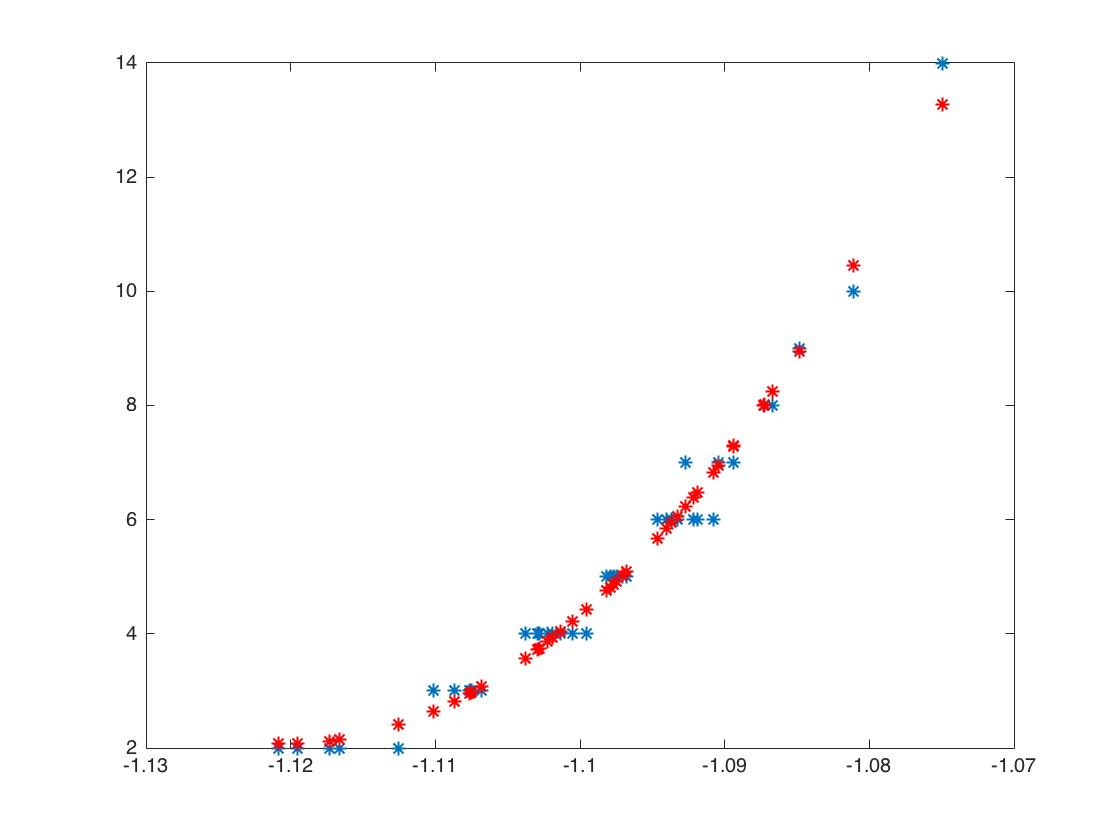
\includegraphics[scale=0.25]{distance_plot}
\end{center}

\section {Code Execution}
Please put test images into \textbf{Test\_set} folder and execute \textbf{code.m} in the submitted project. My algorithm is in \textbf{detect\_barrel.m}. This function has 5 return values.  \textbf{[x,y,d,BW,cc,bb]}. \textbf{x,y} is the centroid, \textbf{d} is the distance. \textbf{BW} is the masked region. \textbf{cc} and \textbf{bb} are the corresponding centroids object and boundingbox objects.  \\
The code will automatically show the detected region and the centroid and print the distance to the matlab \textbf{command line}.\\
The image labeling and model training are in \textbf{labelimages.m} and \textbf{test\_models.m} respectively.
\begin{center}
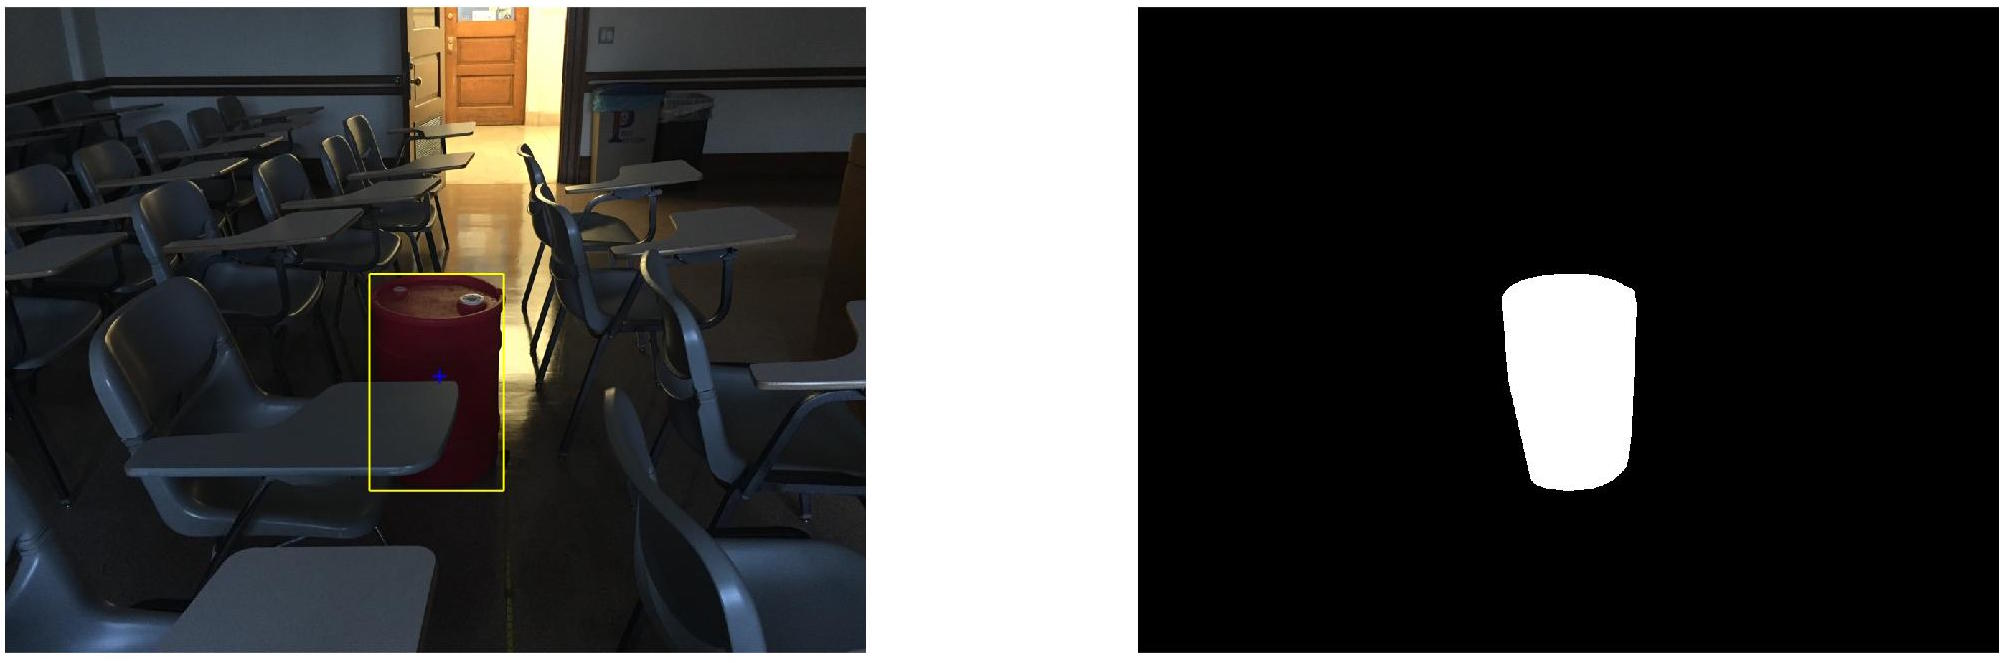
\includegraphics[scale=0.2]{detection_ex1}
\end{center}
\begin{center}
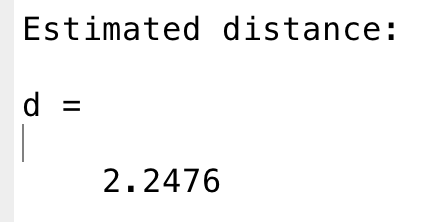
\includegraphics[scale=1]{distance_display}
\end{center}

\end{document}